\chapter{Background}
\label{Chapter4}

In this section we're going to review the concepts required to understand the SVM-RFE algorithm. Section \ref{sec:context} already introduced some concepts around the SVM-RFE algorithm, placed it in context, and enumerated some of its applications. In this section we'll focus on the inner workings of the algorithm and how these parts add together. 

\section{Machine learning}

Machine learning is a subfield in the broader discipline that is artificial intelligence, with a particular take in statistics. These algorithms, also called learning machines or just machines, use data to learn patterns and make predictions. The data is collected in a separated unrelated process, and structured in the form of a \emph{dataset} (a collection of data). Once the dataset is further cleaned and prepared, the learning machine finally consumes it in a process called \emph{training}. After this process the machine pro\-duces a \emph{model}, which is a function that can be used to make predictions on new data.

Two canonical problems in machine learning are regression and classification problems.

\subsection{The dataset}

A dataset is simply a collection of data. In the context of machine learning this data-set will be used to make predictions, take decisions, or find patterns. For a machine learning algorithm to be able to consume a dataset the first step is to represent it in tabular form. 

Most datasets come already in tabular form. Some of the most notable ex\-cep\-tions are datasets involving images. In this case computer vision methods are often used to extract numeric data representing characteristics of the image. Sometimes a more direct transformation can also be made, for example making each feature be the intensity level of a single pixel in the image. This of course produces a high number of features, most of which are redundant or irrelevant (e.g. features representing pixels in the background). 

In a dataset represented as a table, columns describe different \emph{features, properties or attributes} of some group of objects and rows represent \emph{instances} of that group. For example, if objects were vehicles then features could include the brand, power, weight, max\-imum speed, and other such characteristics of various vehicles, each of which would be in a row. Different names are used in different contexts. One of the most typical naming conventions comes from the statistics domain which refers to columns as \emph{variables} and rows as \emph{observations}. Sometimes different nomenclature is used to differentiate features in different stages of the cleaning and preparation process, but in this thesis we use them all instinctively.

\begin{table}[h]
    \makebox[\textwidth][c]{
        \begin{tabular}{l l l l l l l l l}
        \toprule
        \tabhead{Src} & \tabhead{Dst} & \tabhead{NAT-Src} & \tabhead{NAT-Dst} & \tabhead{Action} & \tabhead{Sent (B)} & \tabhead{Rcvd. (B)} & \tabhead{Packets} & \tabhead{Elapsed (sec)}\\
        \midrule
        57222 & 53 & 54587 & 53 & allow & 94 & 83 & 2 & 30 \\
        56258 & 3389 & 56258 & 3389 & allow & 1600 & 3168 & 19 & 17 \\
        6881 & 50321 & 43265 & 50321 & allow & 118 & 120 & 2 & 1199 \\
        43537 & 2323 & 0 & 0 & deny & 60 & 0 & 1 & 0 \\
        50002 & 443 & 45848 & 443 & allow & 6778 & 18580 & 31 & 16 \\
        \bottomrule\\
        \end{tabular}
    }
    \caption{Example extracted from the Internet Firewall Data dataset (\cite{ertam_internet_2019}). Only five observations and main variables shown. }
    \label{tab:example_dataset}
\end{table}

\subsection{Classification}

For the classification problem we want to predict in witch group or \emph{class} to assign some new observation. Table \ref{tab:example_dataset} provides an example of what could be a good classification problem. Imagine we are building a firewall and want it to predict if some new packet in the network should be allowed to pass. We could train a classification learning machine with the dataset represented in the table (the full version) and produce a model capable of doing such predictions. Although it is trivial to identify a pattern in the example, it may not be so for real world examples. Automatic \emph{pattern recognition} is key in solving many real world problems, and it is one of the features of these algorithms.

Mathematically, the set of observations is defined as $X = \{\vt{x_1}, \vt{x_2}, \dots, \vt{x_n}\}$ and the set of the corresponding labels or target classes is $y = \{y_1, y_2, \dots, y_n\}$ with every element of this set being some class $y_i = C_k$ of a discrete set of classes with size $K$. For our example, this set would be $C = \{\text{allow}, \text{deny}\}$. Thus, we can describe the goal of a classification problem as assigning some class $C_k$ to an input vector $\vt{x}$.

Although we've used strings to represent classes, part of the preparation process of the dataset involves turning all values into numerical scalars, so our classes would actually be some natural numbers. Also notice that every $\vt{x_i}$ is a vector containing a single numerical value for each feature excluding the label. 

We make a distinction between two-class problems and multi-class problems. Two-class problems typically use $C = \{0, 1\}$ as classes and thus can be modeled with a boolean function or, if a probability is desired, a function that returns values between 0 and 1. This simplifies the model substantially, in fact some learning machines such as the SVM can only work with two-class problems, and use different methods to extend to the multi-class version.

\subsection{Visualization}

A visualization of the problem in some euclidean space is required to understand how most classification algorithms work, and in particular SVM. Typically, clas\-si\-fi\-cation models divide the input vector space\footnote{The euclidean space of minimum dimension containing all possible input vectors $\vt{x}$.} into \emph{decision regions}. The boundaries of such regions are called \emph{decision boundaries} or \emph{decision surfaces}. If the decision boundary is in the form of some hyperplane of dimension $(D - 1)$, with $D$ being the dimension of the space, then we say that it's a linear model. A dataset whose classes can be completely separated by such linear decision boundary is said to be \emph{linearly separable}.

\begin{figure}[H]
    \centering
    \begin{subfigure}[b]{0.4\linewidth}
        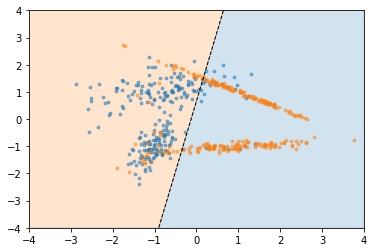
\includegraphics[width=\linewidth]{img/ch4/nolinsep.png}
        \subcaption*{Not linearly separable}
    \end{subfigure}
    \begin{subfigure}[b]{0.4\linewidth}
        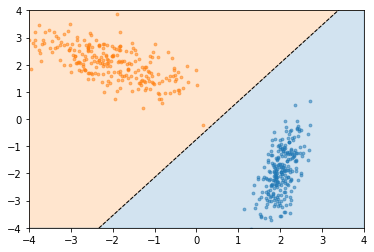
\includegraphics[width=\linewidth]{img/ch4/linsep.png}
        \subcaption*{Linearly separable}
    \end{subfigure}
    \caption{Decision regions and 1-D hyperplane boundary of some linear model for two datasets. Points are observations, colors indicate the class.}
    \label{fig:ch4.sep}
\end{figure}

\subsection{Performance}

\subsection{Microarray Analysis}

\subsubsection{EXTRA}

\emph{Talk about tagging data, unsupervised (clusetring) vs suppervised problems, regression vs classification, dimensions and representation in space, and visualizationa and microarray analysis}

\emph{On Regression and Classification, talk about parameters and hyperparameters, statistical models, mathematical expression and test and training sets, etc}

----------------------------

\begin{itemize}
    \item What is machine learning.
    \item Regression.
    \item Classification.
    \item The dataset, cleaning, embeddings, etc.
\end{itemize}

\section{Support Vector Machines}

\begin{itemize}
    \item 2D classification example.
    \item Mathematical formulation as an optimization problem.
    \item Dual
    \item SVM with regularization.
    \item Dual
    \item Optimization algorithms.
\end{itemize}

\section{Kernel Methods}

\begin{itemize}
    \item What is a kernel.
    \item The kernel trick.
\end{itemize}

\section{SVM-RFE}
\begin{itemize}
    \item What is RFE.
    \item The ranking criteria for the linal case.
\end{itemize}

\begin{algorithm}[H]
    \DontPrintSemicolon
      %\KwInput{$p$}
      \KwOutput{$\vt{r}$}
      \KwData{$X_0,\vt{y}$}
      $\vt{s} = [1,2, \dotsc, n]$ \tcp*{subset of surviving features}
      $\vt{r} = []$ \tcp*{feature ranked list} 
      \While{$|\vt{s}| > 0$}
        {
            \tcc*[h]{Restrict training examples to good feature indices}\\
            $X=X_0(:,\vt{s})$\VS

            \tcc*[h]{Train the classifier}\\
            $\vt{\alpha} = \texttt{SVM-train(} X, y \texttt{)}$\VS

            \tcc*[h]{Compute the weight vector of dimension length $|\vt{s}|$}\\
            $\vt{w} = \sum_k{\vt{\alpha_k} \vt{y_k} \vt{x_k}}$\VS

            \tcc*[h]{Compute the ranking criteria}\\
            $\vt{c} = [(w_i)^2 \text{ for all $i$}]$\VS

            \tcc*[h]{Find the feature with the smallest ranking criterion}\\
            $f = \texttt{argmin($\vt{c}$)}$\VS

            \tcc*[h]{Update the feature ranking list}\\
            $\vt{r} = [\vt{s}(f), ...\vt{r}]$\VS

            \tcc*[h]{Eliminate the feature with smallest ranking criterion}\\
            $\vt{s} = [...\vt{s}(1:f - 1), ...\vt{s}(f + 1:|\vt{s}|)]$
        }
    \caption{SVM-RFE}
\end{algorithm}

\begin{algorithm}[H]
    \DontPrintSemicolon
      \KwInput{$t$ \tcp*{t = step}}
      \KwOutput{$\vt{r}$}
      \KwData{$X_0,\vt{y}$}
      $\vt{s} = [1,2, \dotsc, n]$ \tcp*{subset of surviving features}
      $\vt{r} = []$ \tcp*{feature ranked list} 
      \While{$|\vt{s}| > 0$}
        {
            \tcc*[h]{Restrict training examples to good feature indices}\\
            $X=X_0(:,\vt{s})$\VS

            \tcc*[h]{Train the classifier}\\
            $\vt{\alpha} = \texttt{SVM-train(} X, y \texttt{)}$\VS

            \tcc*[h]{Compute the weight vector of dimension length $|\vt{s}|$}\\
            $\vt{w} = \sum_k{\vt{\alpha_k} \vt{y_k} \vt{x_k}}$\VS

            \tcc*[h]{Compute the ranking criteria}\\
            $\vt{c} = [(w_i)^2 \text{ for all $i$}]$\VS

            \tcc*[h]{Find the $t$ features with the smallest ranking criterion}\\
            $\vt{f} = \texttt{argsort}(\vt{c})(\ :t)$\VS

            \tcc*[h]{Update the feature ranking list}\\
            $\vt{r} = [\vt{s}(\vt{f}), ...\vt{r}]$\VS

            \tcc*[h]{Eliminate the features with the $t$ smallest ranking criterion}\\
            $\vt{s} = [[...\vt{s}(1:f_i - 1), ...\vt{s}(f_i + 1:|\vt{s}|)]$ for all $i]$
        }
    \caption{SVM-RFE with Step}
\end{algorithm}
